\chapter{Simulation}
The simulation consists of a watermark benchmark \cite{watermark15} and a SNR driven Gaussian white noise added to the sum of the signals.
\section{Watermark}
The Watermark Simulation consists of a convolution or channel replay by an selected channel TVIR estimate. The channels consist of multiple dirac impulses of different strengths. Thus, reflections and reduced signal strength are simulated.\


\begin{equation}
	x_{tSigTBr}[k]=\sum_{i=0}^{N}h[k,i]\cdot x_{tSigTB}[k-i]
\end{equation}

\section{White Noise}
A additive Gaussian White Noise (GWN) generated by a desired Signal to Noise Ratio (SNR) between $-20dB$ and $20dB$ in steps of $5dB$. From the general equation of the Signal to Noise Ratio we derive our noise standard deviation by transforming this ratio. The white noise is added after the simulation and before receiver filtering. To estimate the power of our signal a standard deviation estimation is used, which consists of all incoming signals by using its expected value. The Gaussian noise is generated by using a normal distributed random variable with its mean at zero and its standard deviation at $\frac{\bar{\sigma}}{SNR}$. Thus, $M$ denotes the number of total anchors and $N$ is the length of the corresponding signal.

\begin{equation}	
	\bar{\sigma}=\cfrac{1}{M}\sum_{i=0}^{M}\sigma_i,~~~\sigma_j=\sum_{k=0}^{N}{tSigTBr_j}^2[k]
\end{equation}


\begin{equation}
	n[k]=f_{GWN}[k]\cdot \cfrac{\bar{\sigma}}{SNR},~~~GWN\sim\text{Normal}(0,1)
\end{equation}

\begin{figure}[h]
	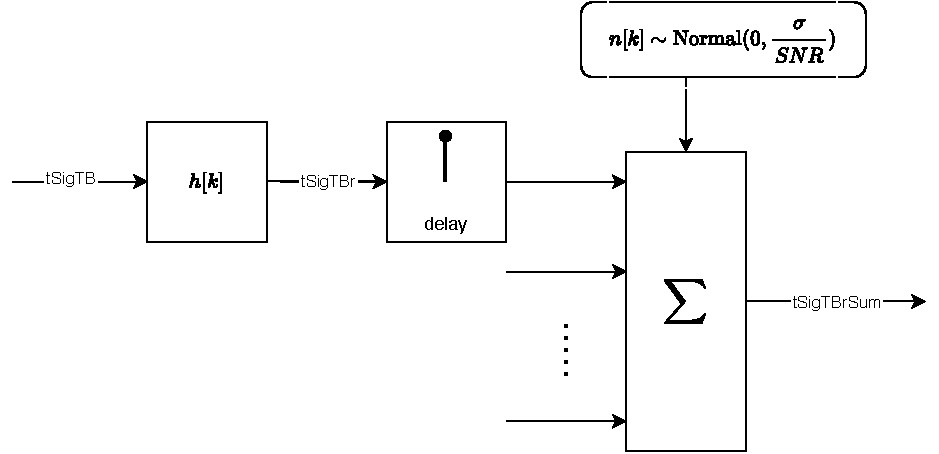
\includegraphics[width=\linewidth]{images/simsig}
	
	\caption{Simulation of acoustic signal propagation}
	\label{fig:simsig}
\end{figure}
